\documentclass[a4paper, 14pt]{extarticle}
\usepackage[utf8]{inputenc}
\usepackage[paper=a4paper, top=1cm, right=1cm, bottom=1.5cm, left=2cm]{geometry}
\usepackage{setspace}
\onehalfspacing

\usepackage{graphicx}
\graphicspath{{plots/}, {images/}}

\parindent=1.25cm

\usepackage{titlesec}

\titleformat{\section}
    {\normalsize\bfseries}
    {\thesection}
    {1em}{}

\titleformat{\subsection}
    {\normalsize\bfseries}
    {\thesubsection}
    {1em}{}

% Настройка вертикальных и горизонтальных отступов
\titlespacing*{\chapter}{0pt}{-30pt}{8pt}
\titlespacing*{\section}{\parindent}{*4}{*4}
\titlespacing*{\subsection}{\parindent}{*4}{*4}

\usepackage[square, numbers, sort&compress]{natbib}
\makeatletter
\bibliographystyle{unsrt}
\renewcommand{\@biblabel}[1]{#1.} 
\makeatother


\newcommand{\maketitlepage}[6]{
    \begin{titlepage}
        \singlespacing
        \newpage
        \begin{center}
            Министерство образования и науки Российской Федерации \\
            Федеральное государственное бюджетное образовательное \\
            учреждение высшего профессионального образования \\
            <<Волгоградский государственный технический университет>> \\
            #1 \\
            Кафедра #2
        \end{center}


        \vspace{14em}

        \begin{center}
            \large Семестровая работа #6 по дисциплине
            \\ <<#3>>
        \end{center}

        \vspace{5em}

        \begin{flushright}
            \begin{minipage}{.35\textwidth}
                Выполнила:\\#4
                \vspace{1em}\\
                Проверил:\\#5
                \\
                \\ Оценка \underline{\ \ \ \ \ \ \ \ \ \ \ \ \ \ \ \ }
            \end{minipage}
        \end{flushright}

        \vspace{\fill}

        \begin{center}
            Волгоград, \the\year
        \end{center}

    \end{titlepage}
    \setcounter{page}{2}
}

\newcommand{\maketitlepagewithvariant}[7]{
    \begin{titlepage}
        \singlespacing
        \newpage

        \begin{center}
            Министерство образования и науки Российской Федерации \\
            Федеральное государственное бюджетное образовательное \\
            учреждение высшего профессионального образования \\
            <<Волгоградский государственный технический университет>> \\
            #1 \\
            Кафедра #2
        \end{center}


        \vspace{8em}

        \begin{center}
            \large Семестровая работа #6 по дисциплине
            \\ <<#3>>
        \end{center}

        \vspace{1em}
        \begin{center}
            Вариант №#7
        \end{center}
        \vspace{4em}

        \begin{flushright}
            \begin{minipage}{.35\textwidth}
                Выполнила:\\#4
                \vspace{1em}\\
                Проверил:\\#5
                \\
                \\ Оценка \underline{\ \ \ \ \ \ \ \ \ \ \ \ \ \ \ \ }
            \end{minipage}
        \end{flushright}

        \vspace{\fill}

        \begin{center}
            Волгоград, \the\year
        \end{center}

    \end{titlepage}
    \setcounter{page}{2}
}

\input{../../.preambles/10-russian}
\input{../../.preambles/20-math}

\newcommand{\ds}{\displaystyle}

\begin{document}
\maketitlepagewithvariant{Факультет электроники и вычислительной техники}
{высшей математики}{Теория вероятности и математическая статистика}{студент
группы Ф-369\\Чечеткин~И.~А.}{Шушков~В.~И.}{\!\!}{15}

\emph{1. Из полного набора костей домино наудачу выбираются четыре. Найти вероятность
того, что ни одна из них не содержит шестерки.}

\vspace*{2em}
\emph{Решение:}

Всего 28 костей, костей с шестеркой -- 7. Тогда искомая вероятность равна
отношению количества сочетаний из 21 по 4 к количеству сочетаний из 28 по 4:
\[
    P = \frac{C_{21}^4}{C_{28}^4} = \frac{21!24!}{17!28!} = \frac{19}{65} = 0,292.
\]

\vspace*{2em}
\emph{Ответ:} \( P = 0,292 \).

\vspace*{2em}

\emph{2. В записной книжке три последние цифры телефонного номера стерлись. В
предположении, что все комбинации трех стершихся цифр равновозможны, найти
вероятность того, что точно две из стершихся цифр совпадают.}

\vspace*{2em}
\emph{Решение:}

Общее количество комбинации: 1000. Количество комбинаций, содержащих две
одинаковые цифры: \( 3\cdot 3^2 \cdot 10 = 270 \).

Используя классическое определение вероятности:
\[
    P = \frac{270}{1000} = 0,27.
\]

\vspace*{2em}
\emph{Ответ:} \( P = 0,27 \).

\pagebreak

\emph{3. Электрическая цепь составлена по схеме, приведенной на рисунке. События
\( A \), \( B_k \) и \( C \) означают исправность элементов \( a \), \( b_k \)
\( (k = 1, 2) \) и \( c \) соответственно.}

\begin{figure}[h!]
    \center
    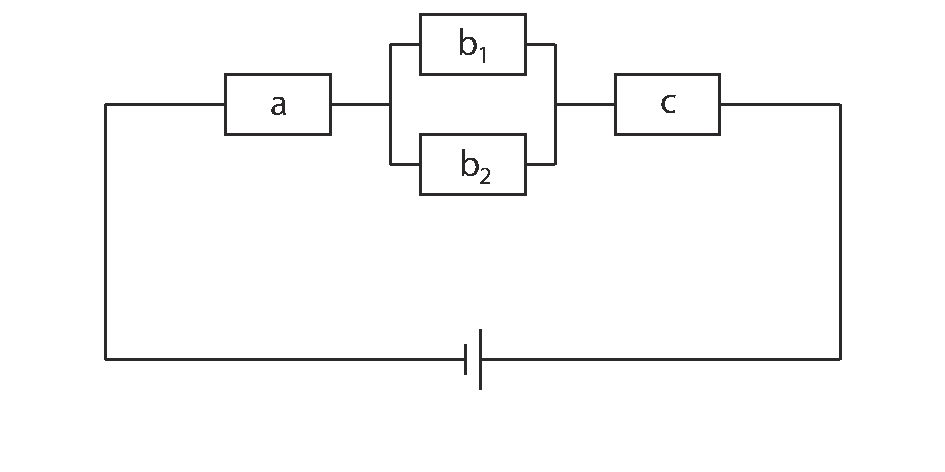
\includegraphics[width=.5\textwidth]{15_3}
\end{figure}

\emph{Выразить событие \( D \) через \( A \), \( B_k \) и \( C \), если \( D \) -- разрыв цепи.}

\vspace*{1em}
\emph{Решение:}

Разрыв цепи произойдет, когда будет не работать элемент \( a \), или элемент
\( c \), или оба элемента \( b_k \):
\[
    D = \bar{A} + \bar{C} + \bar{B}_1\cdot\bar{B}_2.
\]

\vspace*{1em}
\emph{Ответ:} \( D = \bar{A} + \bar{C} + \bar{B}_1\cdot\bar{B}_2 \).

\vspace*{2em}

\emph{4. Стрелок производит три выстрела по мишени. Вероятность попадания в цель при
каждом выстреле равна 0,8. Определить вероятности попадания в цель: \\
1) при всех трех выстрелах; \\
2) при двух выстрелах.}

\vspace*{2em}
\emph{Решение:}

Вероятность попадания в цель при трех выстрелах:
\[
    P_3 = 0,8^3 = 0,512.
\]

Вероятность попадания в цель при двух выстрелах:
\[
    P_2 = (0,8^2 \cdot (1-0,8))\cdot C_3^2 = 3 \cdot 0,128 = 0,384.
\]

\vspace*{1em}
\emph{Ответ:} 1) \( P_3 = 0,512 \), 2) \( P_2 = 0,384 \).

\pagebreak

\emph{5. При включении зажигания двигатель начинает работать с вероятностью 0,9.
Найти вероятности событий: \\ 
\( A \) -- двигатель начнет работать при втором включении зажигания; \\ 
\( B \) -- для запуска двигателя придется включать зажигание не более двух раз.}

\vspace*{2em}
\emph{Решение:}

Если происходит событие \( A \), то это значит, что с первого раза двигатель не
завелся:
\[
    P(A) = 0,9\cdot 0,1 = 0,09.
\]

Наступление события \( B \) означает, что двигатель завелся либо с первого, либо
со второго раза:
\[
    P(B) = 0,9 + 0,9\cdot 0,1 = 0,99.
\]

\vspace*{2em}
\emph{Ответ:} \( P(A) = 0,09 \), \( P(B) = 0,99 \).

\vspace*{2em}

\emph{6. Деталь подвергалась обработке тремя инструментами и в результате оказалась
дефектной. Определить вероятность того, что дефект появился в результате
обработки только вторым инструментом, если вероятности появления дефекта для
каждого из инструментов в отдельности равны соответственно 0,2; 0,1; 0,15.}

\vspace*{2em}
\emph{Решение:}
    
Применяем классическое определение вероятности (\( P_1 = 0,2 \), \( P_2 = 0,1
\), \( P_3 = 0,15 \) -- вероятности появления дефекта для каждого из
инструментов по отдельности):
\begin{align*}
    P = \frac{(1-P_1)P_2(1-P_3)}{P_1P_2P_3 + P_1P_2(1-P_3) + P_1(1-P_2)P_3 +
    (1-P_1)P_2P_3 + \ldots}\\
    \frac{}{\ldots + P_1(1-P_2)(1-P_3) + (1-P_1)P_2(1-P_3) + (1-P_1)(1-P_2)P_3} = 0,175.
\end{align*}
\vspace*{2em}
\emph{Ответ:} \( P = 0,175 \).

\pagebreak

\emph{7. Вероятность появления некоторого события в каждом из пяти независимых опытов
равна 0,7. Найти вероятность появления этого события по крайней мере два раза.}

\vspace*{2em}
\emph{Решение:}

Искомая вероятность является суммой вероятностей тех событий, в которых
вероятное событие наблюдается не менее, чем в двух опытах. По формуле Бернулли
\[
    P_{k,n}=C_n^k\cdot p^k \cdot (1 - p)^{n-k}
\]
имеем
\[
    P = \sum_{k=2}^5 C_5^k 0,7^k (1-0,7)^{5-k} = \sum_{k=2}^5 \frac{5!}{k!(5-k)!}
    0,7^k 0,3^{5-k} = 0,969.
\]

\vspace*{2em}
\emph{Ответ:} \( P = 0,969 \).
\end{document}